%----------------------------------------------------------------------------------------
%    PACKAGES AND THEMES
%----------------------------------------------------------------------------------------

\documentclass[aspectratio=169,xcolor=dvipsnames]{beamer}
\usetheme{SimplePlus}

\usepackage{hyperref}
\usepackage{tikz}
\usepackage{graphicx} % Allows including images
\usepackage{booktabs} % Allows the use of \toprule, \midrule and \bottomrule in tables

%----------------------------------------------------------------------------------------
%    TITLE PAGE
%----------------------------------------------------------------------------------------

\title{0911}
% \subtitle{SUBTITLE}

% \author{AUTHOR}

% \institute
% {
%    DEPARTMENT \\
%    INSTITUTE
% }
\date{\today} % Date, can be changed to a custom date

%----------------------------------------------------------------------------------------
%    PRESENTATION SLIDES
%----------------------------------------------------------------------------------------

\begin{document}

\begin{frame}
    % Print the title page as the first slide
    \titlepage
\end{frame}


%------------------------------------------------
\section{Major Engineering Updates}
%------------------------------------------------

\begin{frame}
    \tableofcontents[currentsection]
\end{frame}

\begin{frame}[allowframebreaks]{Major Engineering Updates}

\textbf{Data, Cache, and Memory Management.}
\begin{itemize}
    \item Construct the data needed for current train-val, save as a local file. (Peak RSS 75\% less, loading time 11 $\to$ 1.85)
    \item Cache certain data, distribute to all algorithms as needed, avoid repeated computation or storage.
    \item Use memory-mapped files to store some precomputed static features, eliminate the copy of large data.
    \item Improve memory management strategy, reduce full-scale memory scan.
    \item Calculating optimization day-to-day, rather than waiting for the whole days' results.
    \item Timely cache release.
\end{itemize}

\break

\textbf{Prediction and Optimization Improvements.}
\begin{itemize}
    \item Change from CPU $\to$ CVXPY $\to$ Clarabel to directly CPU $\to$ Clarabel. (15.66s $\to$ 7.78 s / 600runs)
    \item Opt. problem reuse. E.g., SPO+, each run solves the same problem with only different $\hat{y}$ or $y_{\text{true}}$. Thus, reuse it for Clarabel: \texttt{solver = build\_solver(P, A, b, cones, q\_pred);} \texttt{result\_pred = solver.solve();} \texttt{solver.update(q=q\_true);} \texttt{result\_true = solver.solve().} (6\% less time)
    \item Avoid repeated computation of the same $\hat{y}$ or $y_{\text{true}}$ in the same batch for IC, MSE and decision regrets.
\end{itemize}
    
\break
\textbf{Validation and Testing.}
\begin{itemize}
    \item Use sampling validation. From 240 days to only 48 days for validation (for early-stop criteria). 
    \item Reduce auxiliary feasibility check. E.g., for Tracking Error $\text{TE}(w) = \sqrt{(w - w_{\text{bench}})^\top \Sigma (w - w_{\text{bench}})} \leq 4\%$, we do conduct a pre-check for the feasibility for $4\%$ TE. Pre-checking is somehow reasonable to make sure, e.g. SPO $w^*(\hat{y}), w^*(y_{\text{true}})$ solving the same problem rather than relaxing differently. Yet we try to make this procedure efficient.
    \begin{table}
        \centering
        \footnotesize
        \setlength{\tabcolsep}{4pt}
        \begin{tabular}{l r r r r}
            \toprule
            \textbf{Window} & \textbf{\# Stocks} & \textbf{Before} & \textbf{After} & \textbf{Speedup} \\
            \midrule
            2011-06-30 & 903   & 0.487 s  & 0.028 s & 17$\times$ \\
            2017-12-29 & 2,741 & 3.908 s  & 0.091 s & 43$\times$ \\
            2023-12-29 & 4,786 & 13.388 s & 0.173 s & 77$\times$ \\
            2025-12-31 & 4,866 & 14.397 s & 0.176 s & 82$\times$ \\
            \bottomrule
        \end{tabular}
    \end{table}
\end{itemize}

\break

\textbf{Several Takeaways.}
\begin{itemize}
    \item CUDA is needed.
    \begin{table}
        \centering
        \footnotesize
        \setlength{\tabcolsep}{4pt}
        \begin{tabular}{l c c c}
            \toprule
            \textbf{Method} & \textbf{Full CPU} & \textbf{C+G} & \textbf{Reduction} \\
            \midrule
            PTO-MSE & 56.585 s & 37.559 s & \textbf{33.62\%} \\
            SPO+    & 103.634 s & 93.153 s & \textbf{10.11\%} \\
            \bottomrule
        \end{tabular}
    \end{table}
    \item CuClarabel may not outperform. Precision is fine, but speed is not. (e.g., ablation study: 6.64x slower v.s. CPU on HS300, 2.27x slower on CSI1000) (But yet haven't been tested on real pipeline, may be different)
\end{itemize}

\end{frame}

% \begin{frame}[allowframebreaks]{Results}
    
% \end{frame}

%------------------------------------------------
\section{Han Full Campaign: Interim Status}
%------------------------------------------------

\begin{frame}
    \tableofcontents[currentsection]
\end{frame}

\begin{frame}{Han Full Campaign: Sealed Training Coverage}
    \small
    \begin{itemize}
        \item Protocol: nine annual refits (2017--2025), three random seeds,
        and two training objectives: PTO--Pearson IC and SPO+.
        The planned training total is therefore $9\times3\times2=54$ units.
        \item Campaign snapshot: 52 units have sealed \texttt{summary.json}
        artifacts. These are the only units summarized on the following slide.
    \end{itemize}
    \vspace{3pt}
    \begin{table}
        \centering
        \footnotesize
        \setlength{\tabcolsep}{5pt}
        \begin{tabular}{l l c c}
            \toprule
            \textbf{Refit windows} & \textbf{Refit dates} & \textbf{Sealed units} & \textbf{Status} \\
            \midrule
            $w_0$--$w_7$ & 2017--2024 & $8\times3\times2=48$ & complete \\
            $w_8$ & 2025-12-31 & $4/6$ & seed 3 remains in training \\
            \midrule
            Total & 2017--2025 & $52/54$ & interim snapshot \\
            \bottomrule
        \end{tabular}
    \end{table}
    \vspace{3pt}
    \begin{alertblock}{Scope of this update}
    At the training snapshot above, no OOS decisions, return series, transaction costs, or cross-window
    performance aggregates were available. See the subsequent OOS launch register.
    \end{alertblock}
\end{frame}

\begin{frame}{Sealed Units: Training and Validation Diagnostics}
    \small
    Values are descriptive summaries of sealed training artifacts; validation
    regret is used for checkpoint selection and is not an OOS performance result.
    \vspace{3pt}
    \begin{table}
        \centering
        \scriptsize
        \setlength{\tabcolsep}{4pt}
        \begin{tabular}{l r r r r r}
            \toprule
            \textbf{Objective} & \textbf{Units} & \textbf{Median selected} & \textbf{Median stop} & \textbf{Median validation} & \textbf{Cumulative fit} \\
            & & \textbf{epoch} & \textbf{epoch} & \textbf{regret} & \textbf{time (h)} \\
            \midrule
            PTO--Pearson IC & 26 & 11.5 & 26.5 & 1.2073 & 20.1 \\
            SPO+ & 26 & 12.5 & 27.5 & 1.1306 & 67.1 \\
            \midrule
            All sealed units & 52 & 12.0 & 27.0 & 1.1457 & 87.2 \\
            \bottomrule
        \end{tabular}
    \end{table}
    \vspace{2pt}
    \begin{itemize}
        \item Each sealed unit has 48 effective validation dates, zero recorded
        validation failures, and a valid selection record (2,496 validation dates in total).
        \item The artifacts record 496,028 SPO+ training-oracle solves. Across all
        sealed units, 2,622 solver recoveries were recorded and zero unrecovered
        solver failures were recorded.
        \item The reported fit time is the sum across units, rather than elapsed
        wall-clock time for the campaign.
    \end{itemize}
\end{frame}

% Timing snapshot: 52 sealed units, 2026-09-11 13:33 CST.
% Source: han_full_v7_solver_carry/SUMMARY.csv. Means use 26 units per method.
\begin{frame}{Where Does the Fit Time Go?}
    \small Average time per completed fit, in minutes \hfill 26 fits per method
    \vspace{10pt}

    \centering
    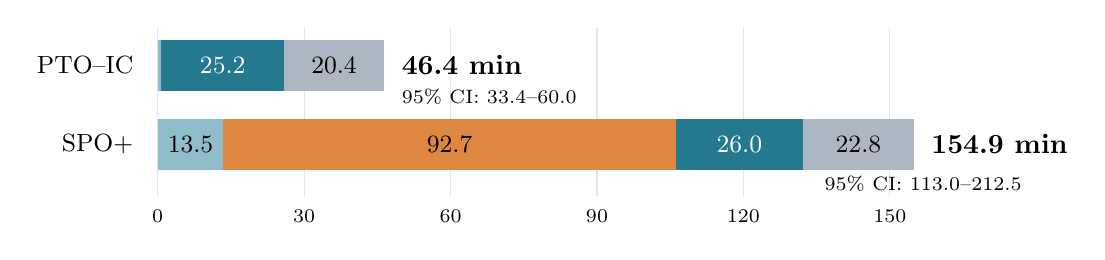
\begin{tikzpicture}[x=0.062cm,y=1cm]
        \definecolor{timeprep}{HTML}{90BDCA}
        \definecolor{timesolve}{HTML}{DE8740}
        \definecolor{timeval}{HTML}{24798E}
        \definecolor{timeother}{HTML}{ADB6C3}
        \foreach \x in {0,30,60,90,120,150} {
            \draw[gray!20] (\x,-0.18)--(\x,1.95);
            \node[font=\scriptsize,anchor=north] at (\x,-0.23) {\x};
        }
        \node[anchor=east,font=\small] at (-3,1.48) {PTO--IC};
        \node[anchor=east,font=\small] at (-3,0.48) {SPO+};
        \fill[timeprep] (0,1.15) rectangle (0.742,1.8);
        \fill[timeval] (0.742,1.15) rectangle (25.917,1.8);
        \fill[timeother] (25.917,1.15) rectangle (46.352,1.8);
        \node[white,font=\small] at (13.33,1.48) {25.2};
        \node[font=\small] at (36.13,1.48) {20.4};
        \node[anchor=west,font=\bfseries] at (48,1.48) {46.4 min};
        \node[anchor=west,font=\scriptsize] at (48,1.08) {95\% CI: 33.4--60.0};
        \fill[timeprep] (0,0.15) rectangle (13.457,0.8);
        \fill[timesolve] (13.457,0.15) rectangle (106.167,0.8);
        \fill[timeval] (106.167,0.15) rectangle (132.151,0.8);
        \fill[timeother] (132.151,0.15) rectangle (154.941,0.8);
        \node[font=\small] at (6.73,0.48) {13.5};
        \node[font=\small] at (59.81,0.48) {92.7};
        \node[white,font=\small] at (119.16,0.48) {26.0};
        \node[font=\small] at (143.55,0.48) {22.8};
        \node[anchor=west,font=\bfseries] at (156.5,0.48) {154.9 min};
        \node[anchor=east,font=\scriptsize] at (179,-0.02) {95\% CI: 113.0--212.5};
    \end{tikzpicture}

    \vspace{6pt}
    {\footnotesize
    \textcolor[HTML]{90BDCA}{\rule{9pt}{9pt}}\ Input preparation\quad
    \textcolor[HTML]{DE8740}{\rule{9pt}{9pt}}\ Training solver\quad
    \textcolor[HTML]{24798E}{\rule{9pt}{9pt}}\ Validation\quad
    \textcolor[HTML]{ADB6C3}{\rule{9pt}{9pt}}\ Other fit work}

    \vspace{7pt}
    \begin{columns}[T,onlytextwidth]
        \begin{column}{0.48\textwidth}
            \textbf{SPO+: 60\% in training solves}\\[3pt]
            \small The largest measured component is the portfolio solver.
        \end{column}
        \begin{column}{0.48\textwidth}
            \textbf{PTO--IC: 54\% in validation}\\[3pt]
            \small Validation takes about 25 minutes for either method.
        \end{column}
    \end{columns}
    \vspace{8pt}
    \raggedright\scriptsize
    95\% percentile CIs: 20,000 refit-window cluster bootstrap draws (9 windows, 26 fits/method).
    Fits have different stopping epochs. These intervals describe between-window variation; overlapping windows limit independence.
\end{frame}

\begin{frame}{Fit Time by Stage: Mean and 95\% Confidence Interval}
    \small Minutes per completed fit \hfill PTO--IC: 26 fits \quad SPO+: 26 fits
    \vspace{5pt}
    \begin{center}
    \renewcommand{\arraystretch}{1.02}
    \begin{tabular}{l r r}
    \toprule
    \textbf{Stage} & \textbf{PTO--IC} & \textbf{SPO+} \\
    \midrule
Data / feature construction & 0.74 [0.55, 0.93] & 0.74 [0.52, 0.98] \\
Optimization problem construction & -- & 12.72 [9.19, 17.77] \\
Prediction (forward pass) & 4.43 [3.24, 5.84] & 4.71 [3.39, 6.95] \\
Backpropagation & 11.27 [8.24, 14.82] & 12.60 [9.09, 18.32] \\
Training solver & -- & 92.71 [69.36, 124.38] \\
Parameter update / gradient handling & 0.15 [0.13, 0.18] & 0.15 [0.13, 0.19] \\
Validation (total) & 25.17 [17.35, 33.17] & 25.98 [16.74, 38.07] \\
Other fit work & 4.58 [3.56, 5.53] & 5.34 [4.20, 6.48] \\
    \midrule
    \textbf{Complete fit} & \textbf{46.35 [33.42, 60.00]} & \textbf{154.94 [113.03, 212.46]} \\
    \bottomrule
    \end{tabular}
    \end{center}
    \vspace{3pt}
    \scriptsize
    Training phases include nested work; validation uses wall time. Other = remaining fit time. ``--'' = not applicable.\\[2pt]
    95\% CIs: 20,000 window-cluster bootstrap draws, seeds retained. Descriptive; windows overlap. CI endpoints are not additive.
\end{frame}

% BEGIN LIVE INTERIM RESULTS
\begin{frame}{Superseded OOS: Execution Bug Identified}
    \small
    \textbf{Same seeds for both methods: 1 and 2.} Each seed covers the full OOS
    calendar. Statistics below summarize the two seed-level metrics.
    \vspace{2pt}
    \begin{table}
    \centering\small\setlength{\tabcolsep}{6pt}
    \begin{tabular}{l r r r r r}
    \toprule
    & \multicolumn{3}{c}{Annualized net excess return} & Median IR & Median TE \\
    \cmidrule(lr){2-4}
    Method & Median & Mean & Range & & \\
    \midrule
SPO+ & 3.70\% & 3.70\% & 2.53--4.88\% & 0.58 & 6.20\% \\
PTO--IC & 2.71\% & 2.71\% & 1.87--3.54\% & 0.39 & 6.85\% \\
    \bottomrule
    \end{tabular}
    \end{table}
    \vspace{2pt}
    \begin{block}{Withdrawn as a strategy comparison; corrected OOS running}
    Median net excess return: \textbf{3.70\% for SPO+ vs. 2.71\% for PTO--IC}.\\
    Median paired difference: \textbf{+1.00 percentage point per year}.\\
    Seed-level direction is mixed: SPO+ leads in one of the two paired seeds.
    \end{block}
    \vspace{4pt}
    \footnotesize With two seeds, the median equals the mean. PTO seed 3 is not
    finished, so SPO+ seed 3 is excluded from both aggregates. Frequent no-trade
    decisions and carried valuations remain part of these interim results.
\end{frame}

\begin{frame}{Superseded OOS: Paired Diagnostics}
    \small
    \textbf{Annualized net excess return versus 000985.}
    Each completed chain covers 404 decisions and 2,020 daily returns.
    \vspace{7pt}
    \begin{table}
    \centering\small\setlength{\tabcolsep}{7pt}
    \begin{tabular}{l r r r r r}
    \toprule
    Seed & SPO+ & PTO--IC & Difference (pp) & SPO+ IR & PTO IR \\
    \midrule
1 & 4.88\% & 1.87\% & +3.01 & 0.72 & 0.35 \\
2 & 2.53\% & 3.54\% & -1.02 & 0.45 & 0.42 \\
\midrule
Mean (1--2) & 3.70\% & 2.71\% & +1.00 & 0.58 & 0.39 \\
    \bottomrule
    \end{tabular}
    \end{table}
    \vspace{8pt}
    \begin{block}{Diagnostic values only; corrected OOS running}
    SPO+ is ahead by 3.01 percentage points in seed 1 and behind by
    1.02 points in seed 2. The paired mean difference is +1.00 point per year.
    \end{block}
    \vspace{5pt}
    \footnotesize Seed 3: SPO+ complete; PTO training unfinished, so it is excluded
    from both method means. Means are averages of seed-level metrics, not an ensemble.
    Frequent no-trade decisions and retained asset valuations limit interpretation.
\end{frame}

\begin{frame}{Superseded OOS: Risk and Execution}
    \small Both methods use the same calendar, benchmark, fee policy and
    missing-exit-quote carry rule.
    \vspace{8pt}
    \begin{table}
    \centering\small\setlength{\tabcolsep}{8pt}
    \begin{tabular}{c l r r r r}
    \toprule
    Seed & Method & Realized TE & Excess max DD & Fee drag (pp/yr) & No-trade \\
    \midrule
1 & SPO+ & 6.79\% & -9.03\% & 0.09 & 383/404 \\
1 & PTO--IC & 5.35\% & -9.19\% & 0.59 & 340/404 \\
2 & SPO+ & 5.61\% & -7.09\% & 0.09 & 383/404 \\
2 & PTO--IC & 8.35\% & -16.40\% & 0.17 & 383/404 \\
    \bottomrule
    \end{tabular}
    \end{table}
    \vspace{7pt}
    \begin{itemize}
    \item Large numbers of no-trade decisions retain earlier portfolios.
    These are conditional backtest results, not evidence of normal rebalancing.
    \item Missing stock close returns retain the previous asset valuation.
    Max DD is measured on relative wealth versus the benchmark.
    \end{itemize}
\end{frame}
% END LIVE INTERIM RESULTS

% BEGIN OOS RERUN TIMING
\begin{frame}{Training and OOS Runtime: Matched-Seed Comparison}
    \small
    \textbf{Training: sum over annual refits. OOS: one continuous evaluation chain.}
    \vspace{6pt}
    \begin{table}
    \centering\small\setlength{\tabcolsep}{9pt}
    \begin{tabular}{l r r r r}
    \toprule
    & \multicolumn{2}{c}{Training (hours)} & \multicolumn{2}{c}{OOS (minutes)} \\
    \cmidrule(lr){2-3}\cmidrule(lr){4-5}
    Seed & SPO+ & PTO--IC & SPO+ & PTO--IC \\
    \midrule
1 & 22.37 & 8.20 & 3.16 & 7.37 \\
2 & 19.59 & 6.19 & 4.83 & 8.66 \\
3 & 29.04 & 5.69 (8/9) & 5.81 & -- \\
\midrule
Median (seeds 1--2) & 20.98 & 7.20 & 3.99 & 8.02 \\
    \bottomrule
    \end{tabular}
    \end{table}
    \vspace{6pt}
    \textbf{Training takes hours; full OOS evaluation takes minutes.}
    \vspace{2pt}
    \scriptsize
    Training includes preparation and validation; PTO seed 3 has eight of nine
    refits sealed. All five OOS chains are complete (CPU inference, 404 decisions).\\[3pt]
    Matched-seed means equal medians here. Artifact preflight is excluded.
    Different no-trade counts affect OOS runtime; these are not per-solve timings.
\end{frame}
% END OOS RERUN TIMING

% BEGIN LOG-BARRIER PREFIX DIAGNOSTIC
\begin{frame}{Log-Barrier: Matched-Prefix OOS Diagnostic}
    \small
    \textbf{Seed 1, $w_0$--$w_2$: 146 decisions and 730 common daily returns
    (2018-01-05--2021-01-06).}
    \vspace{3pt}
    \begin{table}
    \centering\scriptsize\setlength{\tabcolsep}{5pt}
    \begin{tabular}{l r r r r r}
    \toprule
    Method & Net cumulative & Annualized relative & TE & IR & Net MDD \\
    \midrule
    Log-barrier & 16.98\% & 0.44\% & 2.30\% & 0.14 & -31.58\% \\
    SPO+ & 29.54\% & 4.04\% & 5.56\% & 0.74 & -29.93\% \\
    PTO--Pearson IC & 20.97\% & 1.61\% & 5.73\% & 0.31 & -33.83\% \\
    \bottomrule
    \end{tabular}
    \end{table}
    \vspace{1pt}
    \begin{table}
    \centering\scriptsize\setlength{\tabcolsep}{7pt}
    \begin{tabular}{l r r r}
    \toprule
    Method & Training total (h, $w_0$--$w_2$) & OOS total (s) & OOS mean (s/decision) \\
    \midrule
    Log-barrier & 12.24 & 262.35 & 1.797 \\
    SPO+ & 4.43 & 20.07 & 0.137 \\
    PTO--Pearson IC & 1.63 & 53.88 & 0.369 \\
    \bottomrule
    \end{tabular}
    \end{table}
    \vspace{2pt}
    \scriptsize
    The common benchmark cumulative return is 15.51\%. The barrier chain records
    125 carried-restricted-exit, 17 optimal, and 4 optimal-inaccurate decisions;
    no solve failure or warning is recorded. OOS timing uses CPU inference on one
    local host; the barrier mean is 13.07$\times$ SPO+ and 4.87$\times$ PTO--Pearson IC.\\[2pt]
    Training timing is descriptive: the barrier fits ran on a GTX 1660 Ti server,
    whereas the peer fits ran on a local RTX 4060. This is a matched-calendar
    prefix diagnostic, not a final full-sample strategy comparison: the artifacts
    share source, dataset, and problem identities, but have different campaign
    protocols and calculated data identities.
\end{frame}
% END LOG-BARRIER PREFIX DIAGNOSTIC

\begin{frame}{OOS Evaluation: Launch Register}
    \footnotesize
    \textbf{Interim evaluation requested on 11 September 2026.}\\[2pt]
    Five complete annual checkpoint chains are selected from the existing fits.
    \vspace{2pt}
    \begin{table}
    \centering
    \begin{tabular}{l l r}
        \toprule
        Method & Seeds & Decisions per chain \\
        \midrule
        SPO+ & 1, 2, 3 & 404 \\
        PTO--Pearson IC & 1, 2 & 404 \\
        \bottomrule
    \end{tabular}
    \end{table}
    \begin{itemize}
        \item Decision dates: 2018-01-04 to 2026-04-29, every five trading days.
        Holdings remain continuous across annual refits.
        \item CPU inference and Direct Clarabel; existing artifact identities,
        portfolio constraints and transaction-fee policy are retained.
        \item PTO seed 3 remains in training. The initial five-chain subset
        does not constitute acceptance of the full six-chain campaign.
    \end{itemize}
    \vspace{4pt}
    \scriptsize Output: \texttt{results/han\_full\_v7\_interim\_oos\_20260911}.\\
    Status: all three SPO+ chains completed 404/404 decisions.\\
    PTO seeds 1--2 completed; paired interim comparison is available.
\end{frame}

\begin{frame}{OOS Missing Quotes: Continue Without Trading}
    \small
    \textbf{Observed issue.} At the first missing-quote stop, 40 excluded
    holdings lacked execution quotes. The source contains no market rows for
    these stocks around that date; 38 have no records after 2021-08-25.
    \vspace{2pt}
    \begin{itemize}
        \item Existing positions can remain after earlier trading restrictions;
        leaving the optimization universe does not itself liquidate a position.
        \item Adopted interim rule: retain all holdings and skip that rebalance
        when an exit quote is missing. Record the date, affected securities,
        and weights; retry at the next scheduled decision.
        \item No turnover fee is charged for the skipped trade. Missing stock
        close returns retain the previous asset valuation; other holdings
        continue to be valued normally.
    \end{itemize}
    \vspace{2pt}
    \begin{block}{How the results will be reported}
    Disclose missing-quote carry counts and affected holdings alongside returns.
    Retained valuations are assumptions, not observed transaction prices.
    The market-data files alone do not establish the corporate-event cause.
    \end{block}
\end{frame}

\begin{frame}{Remaining Gates Before Results Reporting}
    \small
    \begin{enumerate}
        \item Seal the remaining $w_8$, PTO seed-3 training unit.
        \item Produce OOS decisions under the fixed portfolio and numerical policy.
        \item Aggregate OOS return, turnover, transaction-cost, risk, and
        constraint diagnostics across all annual refits and seeds.
        \item Check campaign identity and completeness before making any
        comparative performance statement.
    \end{enumerate}
    \vspace{8pt}
    \begin{block}{Interpretation}
    The present evidence supports a progress and numerical-stability update only.
    It does not support a conclusion about economic performance or the relative
    effectiveness of PTO--Pearson IC and SPO+.
    \end{block}
\end{frame}


% \section{Small-Data Pipeline}

% \begin{frame}
%     \tableofcontents[currentsection]
% \end{frame}



% \begin{frame}[allowframebreaks]{Motivation and Settings}
%     \begin{itemize}
%         \item Motivation: To construct a small-data pipeline that can be used for quick prototyping and testing of new ideas.
%     \end{itemize}

% \end{frame}







\section{Theoretical discussion: Log-Barrier}

\begin{frame}
    \tableofcontents[currentsection]
\end{frame}
    
\begin{frame}{Pipeline Recap: Prediction Module}

    \begin{itemize}
        \item At day $t$, given 30 historical days' data, totally $m_t$ stocks, each has six features, we have feature tensor $\mathsf{X}_t \in \mathbb{R}^{m_t\times 30 \times 6}$  \footnote{Technically, all prices are divided by the closed price at trade day $t$, and similar to turnover}, and the corresponding label $\mathbf{y}_t \in \mathbb{R}^{m_t}$.
        \item For stock $i$ at day $s$, let $r_{i,s} = \text{adjclose}_{i,s} / \text{adjpreclose}_{i,s} -1$. Then accumulate for the next future 21 days: $R_{i,t} = \prod_{k=2}^{22} (1 + r_{i,t+k}) - 1$. Then 3IQR-standardize + normalize\footnote{Given $R_{i,t}$, 3IQR: denote $\text{IQR} = Q_{.75}-Q_{.25}$, then clip $R_{i,t}$ to $[Q_{.25}-3\text{IQR}, Q_{.75}+3\text{IQR}]$, then normalize by $(R'- \text{mean}(R'))/\text{std}(R')$.} twice, and save as \texttt{float32}. And this is the label $\mathbf{y}_t$.
        \item Then use a GRU to predict each stock a score according to the past 30 days' features, denoted by $\mathbf{s}_t := f_\theta(\mathsf{X}_t) \in \mathbb{R}^{m_t}$, where $|\theta|=62976$. And totally, there are approximately 2380 trade days each window, i.e., $t\in \mathcal{T}_{\text{train}}$ and $|\mathcal{T}_{\text{train}}|=2380$. For each epoch, we randomly sample 200 days (i.e., 200 different $t$'s).
        \item Then normalize $\hat{r}_{i,t} = \frac{s_{i,t} - \bar{s}_t}{\text{std}(\mathbf{s}_t)}$, and this is the input of the optimization problem. 
    \end{itemize}

\end{frame}

\begin{frame}{Pipeline Recap: Optimization Module}
    \small
    Suppress the time subscript. Let $N$ denote the number of stocks
    in the current optimization universe, $\hat r\in\mathbb{R}^N$
    the standardized predicted scores, and
    $w_{\mathrm{prev}},w_b\in\mathbb{R}^N$ the previous portfolio
    and benchmark weights. Define
    \[
    F\in\mathbb{R}^{N\times39},\qquad
    \Sigma_f\in\mathbb{R}^{39\times39},\qquad
    D=\operatorname{diag}(v)\in\mathbb{R}^{N\times N},\qquad
    Q=F\Sigma_f F^\top+D,
    \]
    where $F$ contains stock risk-factor exposures, $\Sigma_f$ is the
    factor covariance matrix, and $D$ contains idiosyncratic variances.
    The vector $\mathbf{1}_{\mathcal B}$ indicates benchmark constituents.

    \[
    \boxed{
    \begin{aligned}
    \max_{w\in\mathbb{R}^N}\quad
    & \hat r^\top w-c\,\lVert w-w_{\mathrm{prev}}\rVert_1 \\[2pt]
    \text{s.t.}\quad
    & \mathbf{1}^\top w=1,\\
    & w^{\min}\leq w\leq w^{\max},\\
    & f^{\min}\leq F^\top(w-w_b)\leq f^{\max},\\
    & (w-w_b)^\top Q(w-w_b)\leq\sigma^2,\\
    & \mathbf{1}_{\mathcal B}^\top w\geq\beta.
    \end{aligned}}
    \]
\end{frame}

\begin{frame}{Optimization Module: Conventions}
    \small
    \begin{itemize}
        \item $N=m_t$ for training and labeled validation cross-sections.
        The OOS optimization universe is not filtered by future-label availability.
        Throughout these slides, $F\in\mathbb{R}^{N\times39}$;
        the implementation stores its transpose.

        \item $w^{\min},w^{\max}$ are effective bounds incorporating
        nonnegativity, the $9\%$ stock-weight cap, benchmark-relative
        bands $w_b\pm0.02$, and price-limit/suspension adjustments.
        Since $w^{\min}\geq0$, a separate $w\geq0$ constraint is redundant.
        Do not add another barrier for this redundant constraint:
        it changes the objective at finite barrier parameters.

        \item Treat $\sigma$ as the given final risk limit for the current
        optimization, after the prescribed TE adjustments.
        The base annual TE limit is $4\%$, with
        $\sigma^2=\sigma_{\mathrm{TE,year}}^2/12$ for the applicable annual limit.

        \item Full turnover is
        $\lVert w-w_{\mathrm{prev}}\rVert_1+T_{\mathrm{out}}$.
        The objective omits the constant $-cT_{\mathrm{out}}$;
        retain it when computing full utility values.

        \item Defaults: $c=0.8$, $\beta=0.8$;
        active style/industry exposure bands: $0.2/0.02$.
    \end{itemize}
\end{frame}

\begin{frame}{Barrier Problem Construction}
    Some preparations:
    \begin{itemize}
        \item Introduce the following slack variables: $s_w^- := w-w^{\min}$, $s_w^+ := w^{\max}-w$, $s_f^- := F^\top(w-w_b)-f^{\min}$, $s_f^+ := f^{\max}-F^\top(w-w_b)$, and $s_{TE} = \sigma^2-(w-w_b)^\top Q(w-w_b)$, $s_{\mathcal{B}} := \mathbf{1}_{\mathcal B}^\top w-\beta$. 
        \item First the $\ell_1$ term is smoothed by: $\Phi_{\delta}(w) := \sum_{i=1}^N \left[\sqrt{(w_i-w_{\mathrm{prev},i})^2+\delta^2}-\delta\right]$.
        \item The log-barrier term is: $\mathcal{B}(w) := \sum_{i=1}^N \left[\log(s_{w,i}^-) + log(s_{w,i}^+)\right] + \sum_{j=1}^{39} \left[\log(s_{f,j}^-) + \log(s_{f,j}^+)\right] + \log(s_{TE}) + \log(s_{\mathcal{B}})$.
    \end{itemize}
    Then the barrier problem is:
    \begin{equation}
    \begin{aligned}
    \max_{w\in\mathbb{R}^N}\quad
    & \hat r^\top w-c\,\Phi_{\delta}(w)+\mu\mathcal{B}(w) \\[2pt]
    \text{s.t.}\quad
    & \mathbf{1}^\top w=1, \quad s_j(w) > 0 \text{ for all } j.
    \end{aligned}
    \end{equation}
    Here $s_j(w)$ denotes the slack variables defined above, and $\mu>0$ is the barrier parameter.
     
\end{frame}

\begin{frame}{Backward Pass: What Are We Differentiating?}
    \small
    The forward pass produces a portfolio. The backward pass asks:
    how should the predicted scores change to improve that portfolio?
    \[
    \theta \longrightarrow \hat r\in\mathbb{R}^N
    \longrightarrow w^\star(\hat r)\in\mathbb{R}^N
    \longrightarrow \mathcal L\in\mathbb{R}.
    \]
    Let $y\in\mathbb{R}^N$ be the observed label vector. Define the
    original portfolio utility and its best feasible portfolio by
    \[
    U_y(w)=y^\top w-c\lVert w-w_{\mathrm{prev}}\rVert_1,
    \qquad w_y^\star\in\arg\max_{w\in\mathcal W}U_y(w),
    \]
    where $\mathcal W$ is the original feasible set. The training loss is
    \[
    \mathcal L=U_y(w_y^\star)-U_y(w^\star(\hat r)),
    \qquad
    g_w:=\frac{\partial\mathcal L}{\partial w^\star}
    =-y+c\,\operatorname{sign}(w^\star-w_{\mathrm{prev}}).
    \]
    The upper loss keeps the original L1 turnover; smoothing is used in
    the lower problem. At zero turnover, use the subgradient $0$.
    The common constant $-cT_{\mathrm{out}}$ cancels in this regret.
    \medskip

    For this backward pass, hold $y$, $w_{\mathrm{prev}}$, the constraints,
    $\mu$, and $\delta$ fixed. The oracle term is then constant with respect
    to $\hat r$; gradients do not continue into previous trading dates.
\end{frame}

\begin{frame}{Backward Pass: Start from the Optimality Conditions}
    \small
    Write the same barrier problem as a minimization:
    \[
    \psi(w;\hat r)=-\hat r^\top w+c\Phi_\delta(w)-\mu\mathcal B(w),
    \qquad \min_{\mathbf1^\top w=1}\psi(w;\hat r).
    \]
    All barrier slacks must be positive. Let $\nu\in\mathbb R$ be the
    multiplier for the sum-to-one constraint. At the solution,
    \[
    \nabla_w\psi(w^\star;\hat r)+\nu^\star\mathbf1=0,
    \qquad \mathbf1^\top w^\star=1.
    \]
    If we slightly change $\hat r$, both $w^\star$ and $\nu^\star$ change.
    Differentiating these two equations gives
    \[
    \underbrace{\begin{bmatrix}H&\mathbf1\\\mathbf1^\top&0\end{bmatrix}}_{K\in\mathbb R^{(N+1)\times(N+1)}}
    \begin{bmatrix}dw^\star\\d\nu^\star\end{bmatrix}
    =\begin{bmatrix}d\hat r\\0\end{bmatrix},
    \qquad H:=\nabla_w^2\psi(w^\star;\hat r).
    \]
    The first row describes how the optimum moves. The second row ensures
    that the change in weights still sums to zero.
\end{frame}

\begin{frame}{Backward Pass: Where Does the Curvature Come From?}
    \small
    The predicted-return term is linear in $w$, so its Hessian is zero.
    Curvature comes from smoothed turnover and the barrier.
    With $d_i=w_i^\star-w_{\mathrm{prev},i}$,
    \[
    c\nabla^2\Phi_\delta(w^\star)
    =c\,\operatorname{diag}\!\left(
    \frac{\delta^2}{(d_i^2+\delta^2)^{3/2}}\right).
    \]
    For each linear slack $s_j$, let $a_j=\nabla s_j$.
    Its contribution to $H$ is $\mu a_ja_j^\top/s_j^2$.
    Let $\mathcal A$ collect these linear slacks and set $x=w^\star-w_b$.
    Including the quadratic TE slack gives
    \[
    \boxed{H=
    c\,\operatorname{diag}\!\left(\frac{\delta^2}{(d_i^2+\delta^2)^{3/2}}\right)
    +\mu\sum_{j\in\mathcal A}\frac{a_ja_j^\top}{s_j^2}
    +\mu\left(\frac{2Q}{s_{TE}}
    +\frac{4(Qx)(Qx)^\top}{s_{TE}^2}\right).}
    \]
    All terms are evaluated at $w^\star$. As a slack gets small, its
    curvature grows: moving towards that boundary becomes harder.
    For $c>0$, $\delta>0$, and $Q\succeq0$, $H$ is positive definite
    at a strictly feasible point.
\end{frame}

\begin{frame}{Backward Pass: One Linear Solve Gives the Gradient}
    \small
    We already have $g_w=\partial\mathcal L/\partial w^\star$.
    We need its effect on the predicted scores, not the full
    $N\times N$ Jacobian of the portfolio.
    Solve the following adjoint system for $v\in\mathbb R^N$ and $q\in\mathbb R$:
    \[
    K^\top\begin{bmatrix}v\\q\end{bmatrix}
    =\begin{bmatrix}g_w\\0\end{bmatrix}.
    \]
    To see why this works, combine it with the previous differential equation:
    \[
    d\mathcal L
    =\begin{bmatrix}g_w\\0\end{bmatrix}^{\!\top}
      \begin{bmatrix}dw^\star\\d\nu^\star\end{bmatrix}
    =\begin{bmatrix}v\\q\end{bmatrix}^{\!\top}
      \begin{bmatrix}d\hat r\\0\end{bmatrix}
    =v^\top d\hat r.
    \]
    Therefore,
    \[
    \boxed{\frac{\partial\mathcal L}{\partial\hat r}=v,\qquad
    \nabla_\theta\mathcal L
    =\left(\frac{\partial\hat r}{\partial\theta}\right)^\top v.}
    \]
    PyTorch passes $v$ through score standardization and the GRU.
    The optimizer then updates $\theta$. We solve a linear system;
    we do not explicitly form a matrix inverse.
\end{frame}

\begin{frame}{Backward Pass: How This Is Used in the Implementation}
    \small
    \begin{enumerate}
        \item Predict $\hat r$, then solve the barrier problem for
        $w^\star$ using CVXPY and Clarabel.
        \item Evaluate the original decision loss and compute $g_w$.
        \item Build the barrier curvature at $w^\star$ and solve for
        the gradient with respect to $\hat r$.
        \item Pass this gradient back through the prediction model.
    \end{enumerate}
    \medskip
    The barrier layer uses an explicit implicit derivative, rather than
    a \texttt{CvxpyLayer} backward call. It differentiates the optimality
    equations at the solution, without unrolling solver iterations.
    \medskip

    The derivation above assumes a strictly feasible point. If a weight
    is fixed by equal bounds, eliminate it first; its zero slacks cannot
    enter a logarithm. Keep any remaining equalities as $Aw=b$.
    For a basis $Z$ of feasible directions ($AZ=0$), the equivalent solve is
    \[
    (Z^\top HZ)u=Z^\top g_w,
    \qquad \frac{\partial\mathcal L}{\partial\hat r}=Zu,
    \]
    expressed in the remaining weight coordinates. This derivative is
    for the current, finite $\mu$ and $\delta$; it is not the derivative
    of the original nonsmooth problem.
\end{frame}













% \begin{frame}{Bullet Points}
%     \begin{itemize}
%         \item Lorem ipsum dolor sit amet, consectetur adipiscing elit
%         \item Aliquam blandit faucibus nisi, sit amet dapibus enim tempus eu
%         \item Nulla commodo, erat quis gravida posuere, elit lacus lobortis est, quis porttitor odio mauris at libero
%         \item Nam cursus est eget velit posuere pellentesque
%         \item Vestibulum faucibus velit a augue condimentum quis convallis nulla gravida
%     \end{itemize}
% \end{frame}

% %------------------------------------------------

% \begin{frame}{Blocks of Highlighted Text}
%     In this slide, some important text will be \alert{highlighted} because it's important. Please, don't abuse it.

%     \begin{block}{Block}
%         Sample text
%     \end{block}

%     \begin{alertblock}{Alertblock}
%         Sample text in red box
%     \end{alertblock}

%     \begin{examples}
%         Sample text in green box. The title of the block is ``Examples".
%     \end{examples}
% \end{frame}

% %------------------------------------------------

% \begin{frame}{Multiple Columns}
%     \begin{columns}[c] % The "c" option specifies centered vertical alignment while the "t" option is used for top vertical alignment

%         \column{.45\textwidth} % Left column and width
%         \textbf{Heading}
%         \begin{enumerate}
%             \item Statement
%             \item Explanation
%             \item Example
%         \end{enumerate}

%         \column{.45\textwidth} % Right column and width
%         Lorem ipsum dolor sit amet, consectetur adipiscing elit. Integer lectus nisl, ultricies in feugiat rutrum, porttitor sit amet augue. Aliquam ut tortor mauris. Sed volutpat ante purus, quis accumsan dolor.

%     \end{columns}
% \end{frame}

% %------------------------------------------------
% \section{SECTION II}
% %------------------------------------------------

% \begin{frame}{Table}
%     \begin{table}
%         \begin{tabular}{l l l}
%             \toprule
%             \textbf{Treatments} & \textbf{Response 1} & \textbf{Response 2} \\
%             \midrule
%             Treatment 1         & 0.0003262           & 0.562               \\
%             Treatment 2         & 0.0015681           & 0.910               \\
%             Treatment 3         & 0.0009271           & 0.296               \\
%             \bottomrule
%         \end{tabular}
%         \caption{Table caption}
%     \end{table}
% \end{frame}

% %------------------------------------------------

% \begin{frame}{Theorem}
%     \begin{theorem}[Mass--energy equivalence]
%         $E = mc^2$
%     \end{theorem}
% \end{frame}

% %------------------------------------------------

% \begin{frame}{Figure}
%     Uncomment the code on this slide to include your own image from the same directory as the template .TeX file.
%     %\begin{figure}
%     %\includegraphics[width=0.8\linewidth]{test}
%     %\end{figure}
% \end{frame}

% %------------------------------------------------

% \begin{frame}[fragile] % Need to use the fragile option when verbatim is used in the slide
%     \frametitle{Citation}
%     An example of the \verb|\cite| command to cite within the presentation:\\~

%     This statement requires citation \cite{p1}.
% \end{frame}

% %------------------------------------------------

\begin{frame}{References}
    \footnotesize
    \bibliography{reference.bib}
    \bibliographystyle{apalike}
\end{frame}

% %------------------------------------------------

% \begin{frame}
%     \Huge{\centerline{\textbf{The End}}}
% \end{frame}

% %----------------------------------------------------------------------------------------

\end{document}
